For the automated analysis, rather than exclusively developing our own tools, we relied as much as 
possible on existing production quality tools and environments.
Our method extracts data about code directly from the production compiler \acs{GCC}, initially with 
an exclusive focus on Fortran, and optionally uses a scalable performance analysis tool (Allinea 
MAP) to obtain information on run-time characteristics.
The optional dynamic analysis is run separately by the user to collect periodic samples of where the 
application is spending time.
These two sources of information are inserted into tables in an \acs{SQL} database, which then 
allows 
for queries to be run using one or both sources of data to gain insight into the code's execution.
An illustration of the this flow can be seen in Figure~\ref{fig:design}.
These steps will be addressed separately in the following subsections.
%While we include components of a dynamic analysis in this way, we primarily emphasise the use of 
%static information, with the dynamic analysis mostly used to narrow the focus more specifically on 
%regions of particular interest and supplement the functional data obtained from the compiler with 
%additional non-functional data obtained from the performance tool.

\begin{figure}
\begin{center}
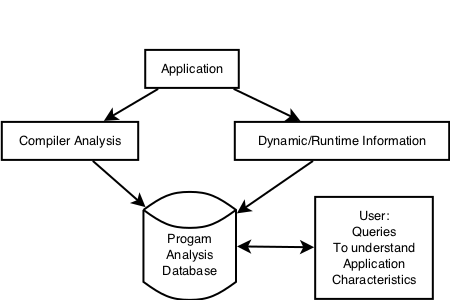
\includegraphics[width=0.45\textwidth]{images/design.png}
\end{center}
\caption{Tool Design}
\label{fig:design}
\end{figure}

The result of this analysis allows users (with optional supplementary run-time data) to get answers to 
questions about applications relevant to their own needs and interests.
We will demonstrate a few examples of this investigative ability in Section~\ref{sec:casestudy}.

\subsection{Static Analysis}
For the static analysis, we relied on \acs{GCC} for its support of Fortran.
Using its plugin \acs{API}, we created a module to be loaded and run after the compiler finishes 
parsing the code.
The plugin runs through all the relevant data structures in the \ac{AST} representing the code to 
queue the data, then proceeds to dump them all at once in bulk transactions.
For the database, we used PostgreSQL for some of its advanced query support.
\subsubsection{Extracting the Static Data}
We did not attempt to create our own schema to represent the code, as it would not immediately be 
necessary due to the tables not being intended as a user-facing interface as well as our current 
focus 
on Fortran not requiring a new language agnostic schema.
%TODO: no possessive acronyms... :'(
Instead, we simply dumped out \acs{GCC}'s internal data structures such that each data structure 
was a table, and each member of the data structure was a column.
We currently extract information from 160 \acs{GCC} data structures (tables) consisting of 1014 
fields (columns).
Eventually, once enough queries have been made for users, it may then be possible to reduce the 
level of information down if there is a great enough difference between what is captured and what is 
actually used, but that is left for future work.
%TODO: technically not all tables...mention enums?
Common to all tables are two columns for the pointer to the data structure in memory during 
compilation, and a build ID unique to each compilation unit.
%TODO: necessary to very briefly explain primary/foreign keys, etc, or are they sufficiently 
%self-describing?
Together, 
%these two fields form the table's composite primary key to uniquely identify each record in 
the database.
Furthermore, this also allows us to dump all data in the most straightforward of manners - primitive 
types get dumped as their corresponding \acs{SQL} data type, and pointers to other objects as the 
raw value of those pointers.

This part of the data can be obtained automatically and without the direct involvement of the user, 
using the same methods used by XALT \cite{7081224}.
That is, a wrapper can be made for \acs{GCC} to intercept compilation and make it use the 
necessary 
plugin, and dump the data either to files, a system log, or directly to the database.
In addition to the primary data about the code itself, XALT is able to insert a unique identifier into 
each 
linked application.
%TODO: expand on the various ID magic
An additional relation between this link ID and the compilation unit build IDs used for each of the files 
being linked must be made so that when applications are run, they can be tied back to each of the 
particular compilations and associated data, which we also need here for connecting the dynamic 
data at a later stage.
\subsubsection{Querying the Static Database}
\label{sec:querying}
Due to the way we identify records and store object references, we are able to use any columns 
representing pointers as foreign keys with which to join connected tables in the database.
One of the most important things we need the database to do for us is associate each code line with 
file lines. A lot of our focus on the analysis is dependent on lines of code, so our queries were 
constructed so as to be able to clearly relate what file and line numbers are involved in an operation.

We are able to use this data to perform the reference counting needed in 
section~\ref{sec:casestudy}.
At a high level, we go through each statement and look up on which files and lines they occur, find all 
references to variables contained in their expression trees, then finally check the symbol table to 
determine which particular variables are being referenced.
We can optionally enhance this further, such as by selecting only variables within particular functions 
of interest, variables of a particular type, variables being assigned to, and/or variables within 
OpenMP regions.
Finally, we can combine the results with that of the dynamic analysis detailed in 
section~\ref{sec:dynamic} so as to know how many times each line was seen in actual execution.
In this way, we are then able to construct queries to tally the total number of references observed for 
every variable across any subset of lines.

In order to ease us in the analysis we performed in section~\ref{sec:casestudy}, we created a couple 
additional virtual tables pieced together from information present in other tables.
Especially important is \texttt{code\_lines}, designed to aid in the process of matching up 
expressions within the code to line numbers and to track which lines come from which subroutine.
Since statements can span multiple lines and source code location is a property of expressions 
rather than statements, we must traverse the expression tree for each statement, find the containing 
line for each expression, then propagate it back up in the reverse direction so that it can be 
aggregated to form the correct line range.
%TODO: given the explanation of the problem, maybe it'd be better to go back and provide a 
%reference to the parent namespace instead of just one of its fields, similar to expr_tree...
The other such table was \texttt{annotated\_code}, which augments \acs{GCC}'s information on code 
lines with an additional two fields for the procedure name's symbol and a list of containing OpenMP 
clauses.

%TODO: keep this or not?
%We initially added some polyhedral analysis information to the database by utilising \acsp{GCC} 
%Graphite framework\cite{trifunovic:inria-00551516}, to do some basic reasoning about memory 
%access 
%order for arrays - notably, to find cases where a particular access is likely to result in either a 
%greater 
%or lesser number of cache misses than a typical in order access pattern.
%However, we determined that there were too many issues with it (e.g. finding good loop candidates 
%for analysis) to be practical at this time, so this was left for future work.

\subsection{Dynamic Analysis}
\label{sec:dynamic}
For the dynamic analysis, we used the ARM MAP sampling based profiler \cite{arm-docs}.
First, given a sample frequency and number of samples, MAP periodically probes the application for 
a set of predetermined metrics, then gathers the samples together to dump them out to an \acs{XML} 
file. Then, in order to link the static and dynamic data later, our tool needs to record the application's 
link ID that was added in during compilation, and a unique run ID for each profile.
What we are interested in is simply where each thread is in the code at the time of sampling, 
specifically the file and line number for each frame of the stack.
We process the \acs{XML} file to extract this information via \ac{XSLT} to produce a \acs{CSV} file 
with the fields we want, and then upload it to the database so that we can obtain a count of how 
many 
times any given line is observed being executed by a thread.
We use this simple metric to determine in what regions of code the application is spending most of 
its time, so that we may focus only upon those regions.

While the static information is dumped once, the dynamic information can be obtained any desired 
number of times.This allows for variable parametres to be used to see their influence on the code, 
such as the number of threads/processes or the problem size. Which profile(s) to use for each 
analysis report must be specified directly by the user upon requesting the report.
The tool can then construct a query that links the compile-time and run-time data based upon the 
application's link ID and MAP run ID(s) to provide the desired results.
